\part{Заміна змінних}
\section{Теоретичні відомості}
\subsection{Основна теорема}
\begin{theorem}
Нехай $A$ --- відкрита підмножина $\eucl{m}$, $B$ --- компактна вимірна підмножина $A$, вектор--функція ${f\colon A\to\eucl{m}}$ задовольняє наступні умови:
\begin{enumerate}
\item відображення $g$ множини $B$ на ${g\left(B\right)}$ взаємно однозначне;
\item вектор--функція $g$ є неперервно диференційовною на $A$;
\item якобіан ${J(y) = g'(y) = \dfrac{\partial\left(g_1,g_2, \ldots, g_m\right)}{\partial\left(y_1,y_2, \ldots, y_m\right)}}$ зберігає знак на $B$, тобто, або ${\forall y\in B\ J(y)>0}$ або ${\forall y\in B\ J(y)<0}$.
\end{enumerate}
Нехай функція ${f\colon g\left(B\right)\to \R}$ неперервна на ${g\left(B\right)}$. Тоді множина ${g\left(B\right)}$ компактна, вимірна і має місце формула
\begin{align*}
\boxed{\int\limits_{g\left(B\right)} f(x) dx = \int\limits_{B} f\left(g\left(y\right)\right) \left|J(y)\right| dx.}
\end{align*}
\end{theorem}
\subsection{Перехід до полярних координат}
Перехід до полярних координат може бути корисним у випадках, коли область інтегрування є колом, або його частиною --- кільцем, сектором, кільцевим сектором. Декартові початкові координати ${\left(x, y\right)}$ виражаються через нові полярні координати ${\left(r, \varphi\right)}$ за допомогою перетворення $g$, що задається формулами
\[
\left(\begin{array}{c}x\\y\end{array}\right) = g\left(r,\varphi\right) =
\left(
\begin{array}{c}
g_1\left(r,\varphi\right)\\
g_2\left(r,\varphi\right)
\end{array}
\right)=
\left(
\begin{array}{c}
r\cos\varphi\\
r\sin\varphi
\end{array}
\right),
\]
тобто
\begin{align*}
x = g_1\left(r, \varphi\right)= r \cos\varphi,\\
y = g_2\left(r, \varphi\right)= r \sin\varphi.
\end{align*}
Якобіан при цьому дорівнює
\begin{align*}
&J(r, \varphi) = \dfrac{\partial\left(g_1,g_2\right)}{\partial\left(r,\varphi\right)} = \begin{vmatrix}\frac{\partial g_1}{\partial r} & \frac{\partial g_1}{\partial \varphi}\\[6pt]\frac{\partial g_2}{\partial r} & \frac{\partial g_2}{\partial \varphi}\end{vmatrix} = \begin{vmatrix}\left(r \cos \varphi\right)'_{r}& \left(r \cos \varphi\right)'_{\varphi}\\[6pt]\left(r \sin \varphi\right)'_{r} & \left(r \sin \varphi\right)'_{\varphi}\end{vmatrix} = \begin{vmatrix}\cos\varphi & -r\sin\varphi\\[6pt]\sin\varphi & r\cos\varphi\end{vmatrix} =&\\&= r \cos^2 \varphi + r \sin^2 \varphi = r.&
\end{align*}

Формула заміни змінних в цьому випадку має наступний вигляд:
\begin{align*}
\boxed{\int\limits_{g\left(B\right)} f(x, y) dx dy = \int\limits_{B} f\left(r \cos \varphi, r \sin \varphi\right) r dr d\varphi.}
\end{align*}

Наведемо в натсупній таблиці декілька прикладів того, як відбувається перетворення областей при переході до полярних координат.

 \begin{longtable}{| @{} m{.30\paperwidth} | m{.30\paperwidth} @{} |}
 \hline
 \bf Початкова область & \bf Нова область \\ \hline \endhead
 \[
   x^2+y^2\leq R
  \]
 &
   \[
   \left\{
   \begin{array}{c}
   0\leq r \leq R, \\
   0 \leq \varphi \leq 2\pi
   \end{array}
   \right.
   \]
   \\*
   \[
   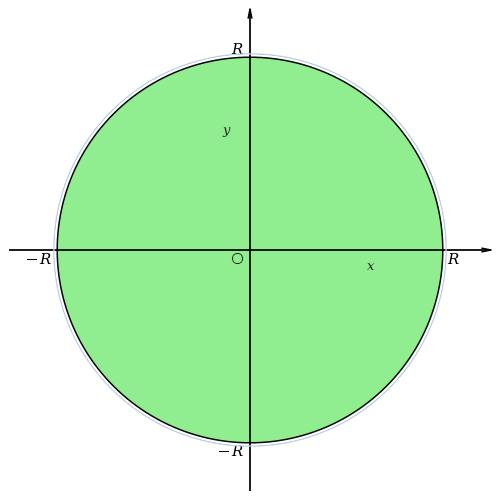
\includegraphics[width=0.2\paperwidth]{change_in_variables_polar_original_circle}
   \]
   &
   \[
   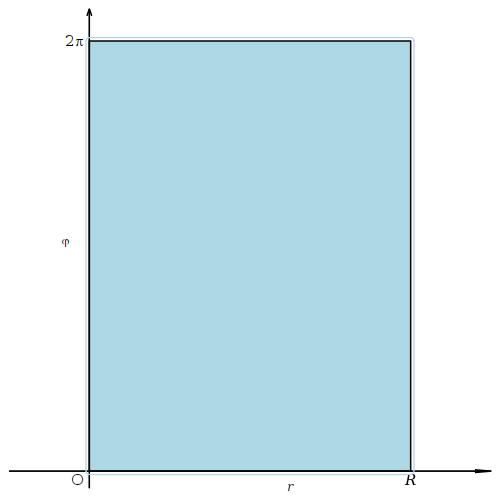
\includegraphics[width=0.2\paperwidth]{change_in_variables_polar_new_circle}
   \]\\
 \hline
   \[
   \left\{
   \begin{array}{c}
   x^2+y^2\leq R,\\
   y\geq 0
   \end{array}
   \right.
   \]
   &
   \[
   \left\{
   \begin{array}{c}
   0\leq r \leq R, \\
   0 \leq \varphi \leq \pi
   \end{array}
   \right.
   \]
   \\*
   \[
   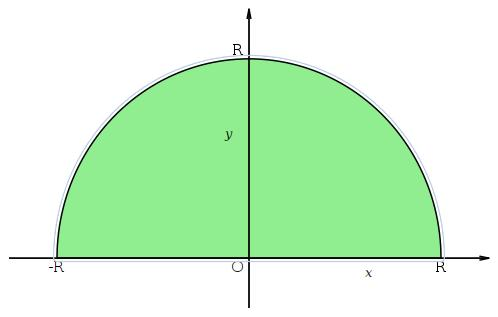
\includegraphics[width=0.2\paperwidth]{change_in_variables_polar_original_upper_semicircle}
   \]
   &
   \[
   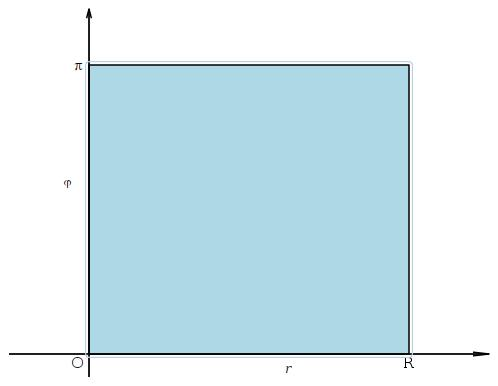
\includegraphics[width=0.2\paperwidth]{change_in_variables_polar_new_upper_semicircle}
   \]
   \\
 \hline
   \[
   \left\{
   \begin{array}{c}
   x^2+y^2\leq R,\\
   y\leq 0
   \end{array}
   \right.
   \]
   &
   \[
   \left\{
   \begin{array}{c}
   0\leq r \leq R, \\
   -\pi \leq \varphi \leq 0
   \end{array}
   \right.
   \]
   \\*
   \[
   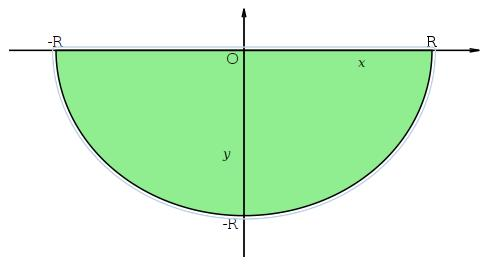
\includegraphics[width=0.2\paperwidth]{change_in_variables_polar_original_lower_semicircle}
   \]
   &
   \[
   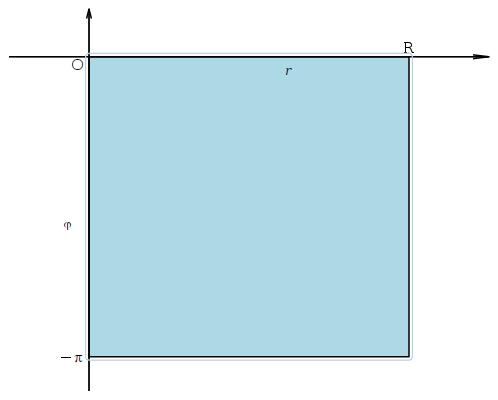
\includegraphics[width=0.2\paperwidth]{change_in_variables_polar_new_lower_semicircle}
   \]
   \\
 \hline
   \[
   \left\{
   \begin{array}{c}
   x^2+y^2\leq R,\\
   x\geq 0
   \end{array}
   \right.
   \]
   &
   \[
   \left\{
   \begin{array}{c}
   0\leq r \leq R, \\
   -\frac{\pi}{2} \leq \varphi \leq \frac{\pi}{2}
   \end{array}
   \right.
   \]
   \\*
   \[
   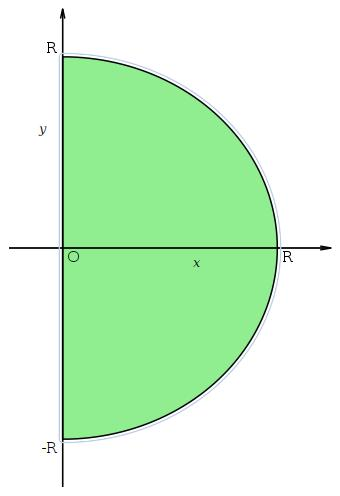
\includegraphics[width=0.2\paperwidth]{change_in_variables_polar_original_right_semicircle}
   \]
  &
   \[
   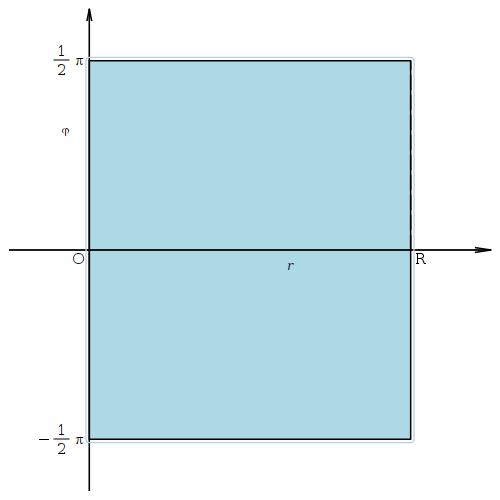
\includegraphics[width=0.2\paperwidth]{change_in_variables_polar_new_right_semicircle}
   \]
   \\
 \hline
 \[
   \left\{
   \begin{array}{c}
   x^2+y^2\leq R,\\
   x\leq 0
   \end{array}
   \right.
   \]
 &
 \[
   \left\{
   \begin{array}{c}
   0\leq r \leq R, \\
   \frac{\pi}{2}\leq \varphi \leq \frac{3\pi}{2}
   \end{array}
   \right.
   \]\\*
   \[
   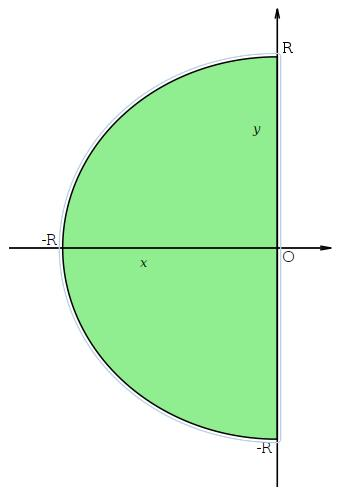
\includegraphics[width=0.2\paperwidth]{change_in_variables_polar_original_left_semicircle}
   \]
   &
   \[
   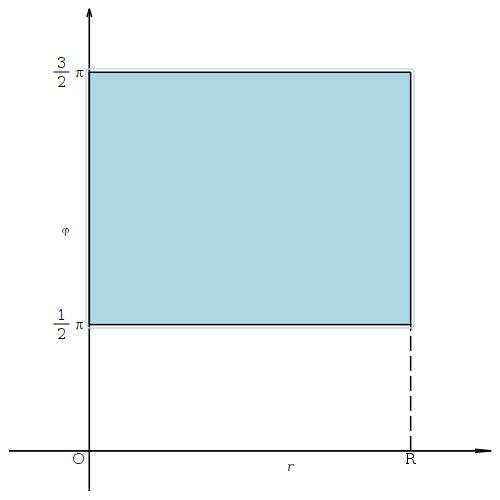
\includegraphics[width=0.2\paperwidth]{change_in_variables_polar_new_left_semicircle}
   \]
   \\
   \hline
   \[
   \left\{
   \begin{array}{c}
   x^2+y^2\leq R,\\
   x\geq 0,\\
   y\geq 0
   \end{array}
   \right.
   \]
   &
   \[
   \left\{
   \begin{array}{c}
   0\leq r \leq R, \\
   0 \leq \varphi \leq \frac{\pi}{2}
   \end{array}
   \right.
   \]
   \\*
   \[
   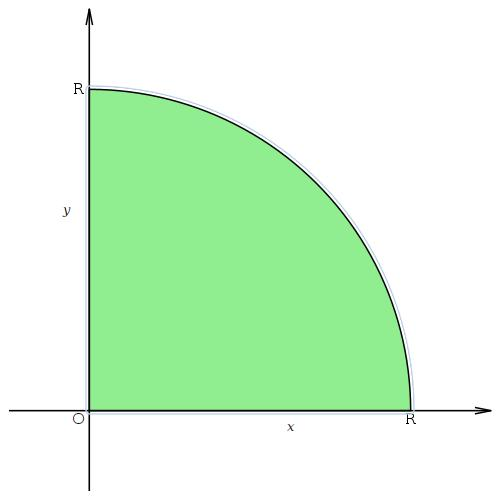
\includegraphics[width=0.2\paperwidth]{change_in_variables_polar_original_1st_quadrant}
   \]
   &
   \[
   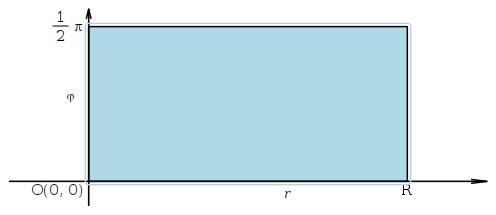
\includegraphics[width=0.2\paperwidth]{change_in_variables_polar_new_1st_quadrant}
   \]
   \\
   \hline
   \[
   \left\{
   \begin{array}{c}
   x^2+y^2\leq R,\\
   x\leq 0,\\
   y\geq 0
   \end{array}
   \right.
   \]
   &
   \[
   \left\{
   \begin{array}{c}
   0\leq r \leq R, \\
   \frac{\pi}{2} \leq \varphi \leq \pi
   \end{array}
   \right.
   \]
   \\*
   \[
   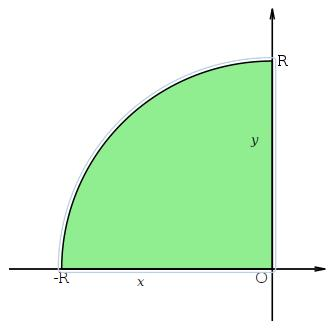
\includegraphics[width=0.2\paperwidth]{change_in_variables_polar_original_2nd_quadrant}
   \]
   &
   \[
   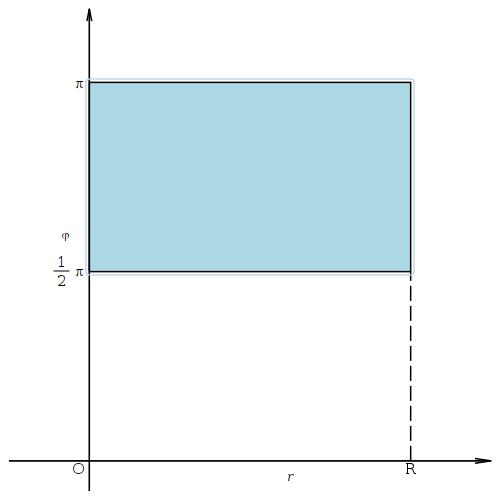
\includegraphics[width=0.2\paperwidth]{change_in_variables_polar_new_2nd_quadrant}
   \]
   \\
   \hline
   \[
   \left\{
   \begin{array}{c}
   x^2+y^2\leq R,\\
   x\leq 0,\\
   y\leq 0
   \end{array}
   \right.
   \]
   &
   \[
   \left\{
   \begin{array}{c}
   0\leq r \leq R, \\
   -\pi \leq \varphi \leq -\frac{\pi}{2}
   \end{array}
   \right.
   \]
   \\*
   \[
   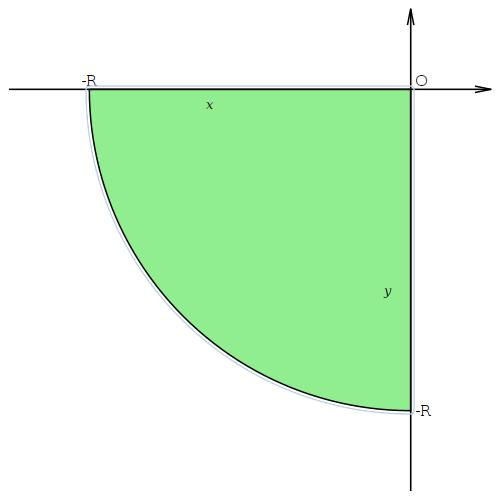
\includegraphics[width=0.2\paperwidth]{change_in_variables_polar_original_3rd_quadrant}
   \]
   &
   \[
   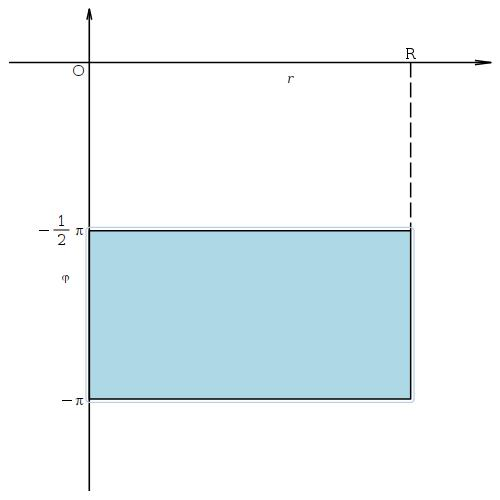
\includegraphics[width=0.2\paperwidth]{change_in_variables_polar_new_3rd_quadrant}
   \]
   \\
   \hline
   \[
   \left\{
   \begin{array}{c}
   x^2+y^2\leq R,\\
   x\geq 0,\\
   y\leq 0
   \end{array}
   \right.
   \]
   &
   \[
   \left\{
   \begin{array}{c}
   0\leq r \leq R, \\
   -\frac{\pi}{2} \leq \varphi \leq 0
   \end{array}
   \right.
   \]
   \\*
   \[
   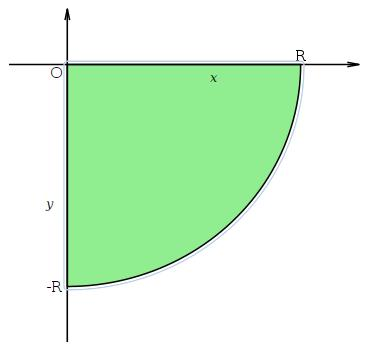
\includegraphics[width=0.2\paperwidth]{change_in_variables_polar_original_4th_quadrant}
   \]
   &
   \[
   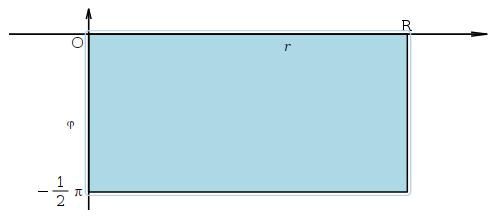
\includegraphics[width=0.2\paperwidth]{change_in_variables_polar_new_4th_quadrant}
   \]
   \\
   \hline
   \[
   \left\{
   \begin{array}{c}
   x^2+y^2\leq R_2,\\
   x^2+y^2\geq R_1,\\
   y\geq x\tg \alpha,\\
   y\geq x\tg \beta
   \end{array}
   \right.
   \]
   &
   \[
   \left\{
   \begin{array}{c}
   R_1\leq r \leq R_2, \\
   \alpha \leq \varphi \leq \beta
   \end{array}
   \right.
   \]
   \\*
   \[
   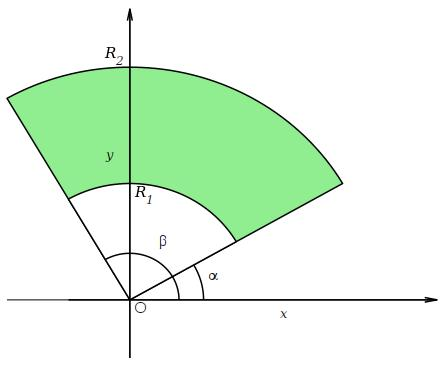
\includegraphics[width=0.2\paperwidth]{change_in_variables_polar_original_ring_sector}
   \]
   &
   \[
   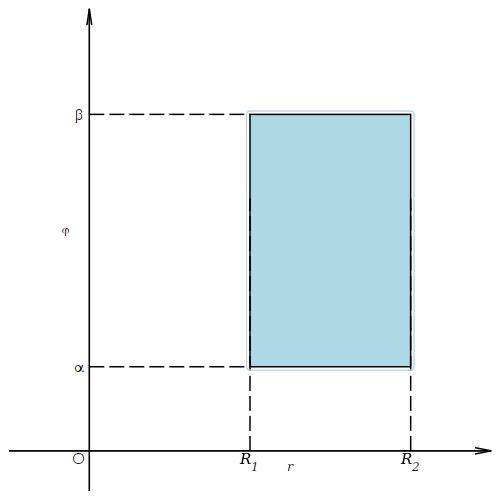
\includegraphics[width=0.2\paperwidth]{change_in_variables_polar_new_ring_sector}
   \]
   \\
   \hline
   \[
   \left\{
   \begin{array}{c}
   x^2+y^2\leq R,\\
   y\geq x\tg \alpha,\\
   y\geq x\tg \beta
   \end{array}
   \right.
   \]
   &
   \[
   \left\{
   \begin{array}{c}
   0\leq r \leq R, \\
   \alpha \leq \varphi \leq \beta
   \end{array}
   \right.
   \]
   \\*
   \[
   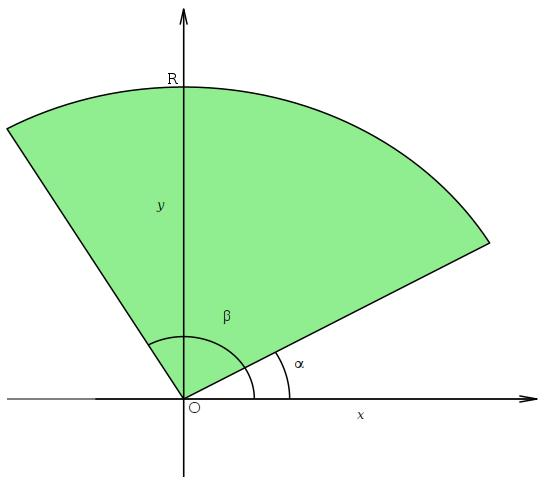
\includegraphics[width=0.2\paperwidth]{change_in_variables_polar_original_sector}
   \]
   &
   \[
   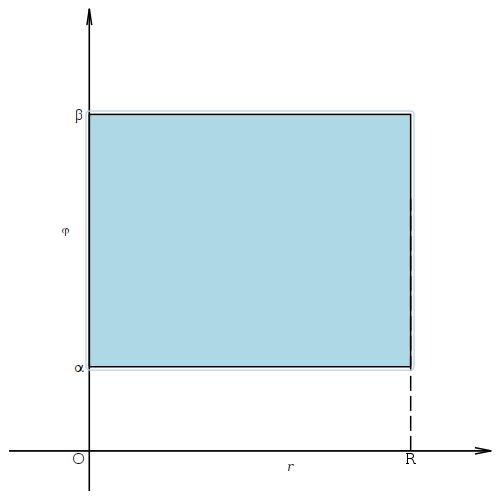
\includegraphics[width=0.2\paperwidth]{change_in_variables_polar_new_sector}
   \]
   \\
   \hline
 \end{longtable}

\subsection{Перехід до сферичних координат}
Перехід до сферичних координат може бути корисним у випадках, коли область інтегрування є тривимірною кулею, або її частиною --- кільцем, сектором, кільцевим сектором. Декартові початкові координати ${\left(x, y, z\right)}$ виражаються через нові сферичні координати ${\left(r, \varphi, \theta\right)}$ за допомогою перетворення $g$, що задається формулами
\[
\left(\begin{array}{c}x\\y\\z\end{array}\right) = g\left(r, \varphi, \theta\right) =
\left(
\begin{array}{c}
g_1\left(r,\varphi. \theta\right)\\
g_2\left(r,\varphi. \theta\right)\\
g_3\left(r,\varphi. \theta\right)\\
\end{array}
\right)=
\left(
\begin{array}{c}
r\cos\theta\cos\varphi\\
r\cos\theta\sin\varphi\\
r\sin\theta
\end{array}
\right),
\]
тобто
\begin{align*}
x = g_1\left(r, \varphi, \theta\right)= r \cos\theta \cos\varphi,\\
y = g_2\left(r, \varphi, \theta\right)= r \cos\theta \sin\varphi,\\
z = g_2\left(r, \varphi, \theta\right)= r \sin\theta.
\end{align*}
Якобіан при цьому дорівнює
\begin{align*}
&J(r, \varphi, \theta) = \dfrac{\partial\left(g_1,g_2,g_3\right)}{\partial\left(r,\varphi,\theta\right)} =
\begin{vmatrix}
\frac{\partial g_1}{\partial r} & \frac{\partial g_1}{\partial \varphi} & \frac{\partial g_1}{\partial \theta}\\[6pt]\frac{\partial g_2}{\partial r} & \frac{\partial g_2}{\partial \varphi} & \frac{\partial g_2}{\partial \theta}\\[6pt]\frac{\partial g_3}{\partial r} & \frac{\partial g_3}{\partial \varphi} & \frac{\partial g_3}{\partial \theta}
\end{vmatrix}
=
\begin{vmatrix}
\left(r \cos\theta \cos \varphi\right)'_{r} & \left(r \cos\theta \cos \varphi\right)'_{\varphi} & \left(r \cos\theta \cos \varphi\right)'_{\theta}\\[6pt]
\left(r \cos \theta \sin \varphi\right)'_{r} & \left(r \cos \theta \sin \varphi\right)'_{\varphi} & \left(r \cos\theta \sin \varphi\right)'_{\theta}\\[6pt]
\left(r \sin \theta\right)'_{r} & \left(r \sin \theta\right)'_{\varphi} & \left(r \sin\theta\right)'_{\theta}\end{vmatrix} = & \\[6pt]
&=
\begin{vmatrix}
\cos\theta \cos \varphi & - r \cos\theta \sin \varphi & - r \sin\theta \cos \varphi\\[6pt]
\cos \theta \sin \varphi & r \cos \theta \cos \varphi & - r \sin\theta \sin \varphi\\[6pt]
\sin \theta & 0 & r \cos\theta
\end{vmatrix}
= \underline{r^2 \cos^2 \varphi \cos^3 \theta} + \underline{\underline{r^2 \sin^2 \varphi \cos \theta \sin^2 \theta}} + & \\[6pt]
& + \underline{r^2 \cos^2 \varphi \sin^2\theta \cos \theta} + \underline{\underline{r^2 \cos^3 \theta \sin^2 \varphi}} = r^2 \cos^2 \varphi \cos \theta \left(\cos^2 \theta + \sin^2 \theta\right) +&\\[6pt]
&+r^2 \sin^2 \varphi \cos \theta \left(\sin^2 \theta +\cos^2 \theta\right) = r^2 \cos^2 \varphi \cos \theta + r^2 \sin^2 \varphi \cos \theta = r^2 \cos \theta \left(\cos^2 \varphi + \sin^2 \varphi \right) = &\\[6pt] & = r^2 \cos \theta.
\end{align*}

Формула заміни змінних в цьому випадку має наступний вигляд:
\begin{align*}
\boxed{\int\limits_{g\left(B\right)} f(x, y, z) dx dy dz = \int\limits_{B} f\left(r \cos\theta \cos\varphi, r \cos\theta \sin\varphi, r \sin\theta \right) r^2 \cos \theta dr d\varphi d\theta.}
\end{align*}
\subsection{Перехід до циліндричних координат}
Перехід до циліндричних координат може бути корисним у випадках, коли область інтегрування є тривимірною циліндричною областю з колом, або його частиною --- кільцем, сектором, кільцевим сектором --- в основі. Декартові початкові координати ${\left(x, y, z\right)}$ виражаються через нові циліндричні координати ${\left(r, \varphi, z\right)}$ за допомогою перетворення $g$, що задається формулами
\[
\left(\begin{array}{c}x\\y\\z\end{array}\right) = g\left(r, \varphi, \theta\right) =
\left(
\begin{array}{c}
g_1\left(r,\varphi. z\right)\\
g_2\left(r,\varphi. z\right)\\
g_3\left(r,\varphi. z\right)\\
\end{array}
\right)=
\left(
\begin{array}{c}
r \cos\varphi\\
r \sin\varphi\\
z
\end{array}
\right),
\]
тобто
\begin{align*}
x = g_1\left(r, \varphi, z\right)= r \cos\varphi,\\
y = g_2\left(r, \varphi, z\right)= r \sin\varphi,\\
z = g_2\left(r, \varphi, z\right)= z.
\end{align*}
Якобіан при цьому дорівнює
\begin{align*}
&J(r, \varphi, z) = \dfrac{\partial\left(g_1,g_2,g_3\right)}{\partial\left(r,\varphi,z\right)} =
\begin{vmatrix}
\frac{\partial g_1}{\partial r} & \frac{\partial g_1}{\partial \varphi} & \frac{\partial g_1}{\partial z}\\[6pt]\frac{\partial g_2}{\partial r} & \frac{\partial g_2}{\partial \varphi} & \frac{\partial g_2}{\partial z}\\[6pt]\frac{\partial g_3}{\partial r} & \frac{\partial g_3}{\partial \varphi} & \frac{\partial g_3}{\partial z}
\end{vmatrix}
=
\begin{vmatrix}
\left(r \cos \varphi\right)'_{r} & \left(r \cos \varphi\right)'_{\varphi} & \left(r \cos \varphi\right)'_{z}\\[6pt]
\left(r \sin \varphi\right)'_{r} & \left(r \sin \varphi\right)'_{\varphi} & \left(r \sin \varphi\right)'_{z}\\[6pt]
\left(z \right)'_{r} & \left(z \right)'_{\varphi} & \left(z\right)'_{z}\end{vmatrix} = & \\[6pt]
&=
\begin{vmatrix}
 \cos \varphi & - r \sin \varphi & 0\\[6pt]
 \sin \varphi & r \cos \varphi & 0\\[6pt]
0 & 0 & 1
\end{vmatrix}
= r \cos^2 \varphi + r \sin^2 \varphi = r.
\end{align*}

Формула заміни змінних в цьому випадку має наступний вигляд:
\begin{align*}
\boxed{\int\limits_{g\left(B\right)} f(x, y, z) dx dy dz = \int\limits_{B} f\left(r \cos\varphi, r \sin\varphi, z \right) r dr d\varphi dz.}
\end{align*}
\section{Приклади обчислень}
\begin{example}[перехід до полярних координат]
Знайти ${\iint\limits_D x y d x d y}$, де через $D$ позначена область в першому квадранті ${x\geq0}$, ${y\geq0}$, що обмежена лініями ${x^2 +y^2 = R^2}$, ${y= 0}$, ${y = x\sqrt{3}}$.
\end{example}
Зробимо рисунок почактової області $D$ (нагадаємо, що ${\sqrt{3} = \tg \frac{\pi}{3}}$):
\[
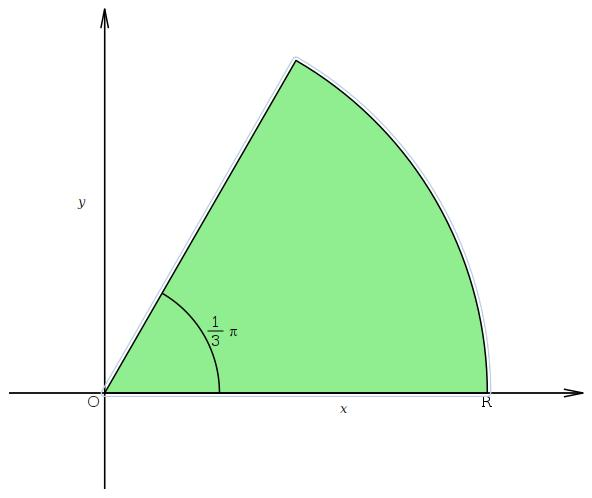
\includegraphics[width=0.3\paperwidth]{change_in_variables_example_polar_original}
\]
Після переходу до полярних координат нова область $D'$ виглядає наступним чином:
\[
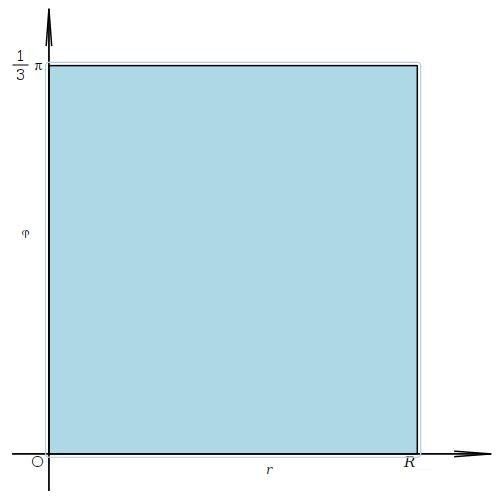
\includegraphics[width=0.3\paperwidth]{change_in_variables_example_polar_new}
\]

\begin{align*}
&\iint\limits_D x y d x d y = \iint\limits_{D'} r \cos \varphi r \cdot \sin \varphi \cdot r d r d \varphi = \int\limits_{0}^{R}\left(\int\limits_{0}^{\frac{\pi}{3}}r^3 \cos \varphi \sin \varphi d \varphi\right) d r =&\\
&= \int\limits_{0}^{R}\left(\frac{1}{2}\int\limits_{0}^{\frac{\pi}{3}}r^3 \sin 2 \varphi d \varphi\right) d r = \int\limits_{0}^{R}\frac{1}{2}\left(-\frac{1}{2}r^3 \cos 2 \varphi \biggr|_{\varphi = 0}^{\frac{\pi}{3}} \right) d r = &\\
&= \int\limits_{0}^{R}\left(-\frac{1}{4}r^3 \cos 2 \frac{\pi}{3} - \left(-\frac{1}{4}r^3 \cos 0\right) \right) d r = \int\limits_{0}^{R}\left(\frac{1}{8}r^3 - \left(-\frac{1}{4}r^3 \right) \right) d r = &\\
& = \int\limits_{0}^{R}\frac{3}{8}r^3 d r = \frac{3}{8}\cdot\frac{r^4}{4}\biggr|_{0}^{R} = \frac{3 R^4}{32} - 0 = \frac{3 R^4}{32}.&
\end{align*}
\begin{example}[Загальна формула]
Знайти ${\iint\limits_D \ln\left(x + y\right) d x d y}$, де через $D$ позначений паралелограм, що обмежений прямими ${x - 3y + 7 = 0}$, ${x - 3y + 2 = 0}$, ${2x - y - 1 = 0}$, ${2x - y - 6 = 0}$.

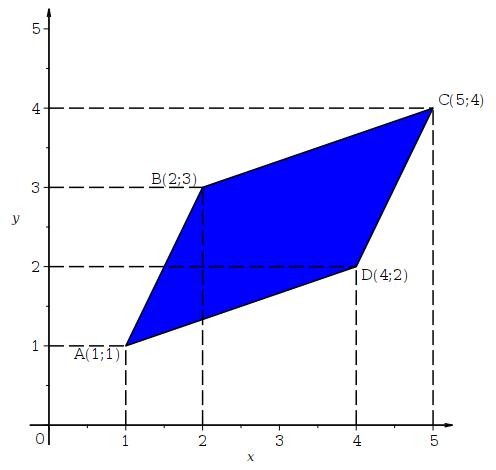
\includegraphics[width=0.5\paperwidth]{example.2.6}

Як і в попередніх прикладах, область $D$ є множиною на площині циліндричною в напрямку осі ${Oy}$. Однак тепер, якщо безпосередньо зводити подвійний інтеграл до повторного, то ми отримаємо суму не двох, а трьох повторних інтегралів:
\[
\begin{array}{l}
\iint\limits_D \ln\left(x + y\right) d x d y =\\= \int\limits_1^2 d x \int\limits_{\frac{x+2}{3}}^{2 x - 1}\ln\left(x + y\right) d y + \int\limits_2^4 d x\int\limits_{\frac{x+2}{3}}^{\frac{x + 7}{3}}\ln\left(x + y\right) d y + \int\limits_4^5 d x\int\limits_{2 x - 6}^{\frac{x + 7}{3}}\ln\left(x + y\right) d y.
\end{array}
\]
\begin{exercise}
Підрахуйте ці повторні інтеграли і переконайтесь, що в сумі ви отримали таку саму відповідь, яку ми отримаємо нижче за допомогою заміни змінних.
\end{exercise}
\begin{exercise}
Зведіть даний в умові подвійний інтеграл до суми трьох повторних на підставі того, що $D$ є множиною циліндричною в напрямку також осі ${Ox}$.
\end{exercise}
Розглянемо нові змінні
\[
\begin{array}{c}
s = 3 y - x,\\
t = 2 x - y.
\end{array}
\]
Фактично ми задали перетворення ${h\colon \eucl{2}\to\eucl{2}}$, яке точку ${\left(x, y\right)\in\eucl{2}}$
 переводить в точку ${\left(s,t\right) = h\left(x,y\right)\in\eucl{2}}$ за наведеними вище формулами. В геометрії такі пертворення називаються афінними. Відомо, що афінні перетворення зберігають паралельність прямих, а тому переводять паралелограми в паралелограми. В нашому випадку область $D$ є паралелограмом з вершинами ${\left(1,1\right)}$, ${\left(2,3\right)}$, ${\left(5,4\right)}$ і ${\left(4,2\right)}$. Знайдемо тепер, в які точки переводить перетворення $h$ вершини нашого паралелограма:
 \[
 \begin{array}{c}
 h\left(1,1\right) = \left(\begin{array}{c}3\cdot1 - 1\\2\cdot 1 - 1\end{array}\right) = \left(\begin{array}{c}2\\1\end{array}\right),\\
 h\left(2,3\right) = \left(\begin{array}{c}3\cdot3 - 2\\2\cdot 2 - 3\end{array}\right) = \left(\begin{array}{c}7\\1\end{array}\right),\\
 h\left(5,4\right) = \left(\begin{array}{c}3\cdot4 - 5\\2\cdot 5 - 4\end{array}\right) = \left(\begin{array}{c}7\\6\end{array}\right),\\
 h\left(4,2\right) = \left(\begin{array}{c}3\cdot2 - 4\\2\cdot 4 - 2\end{array}\right) = \left(\begin{array}{c}2\\6\end{array}\right),\\
 \end{array}
 \]

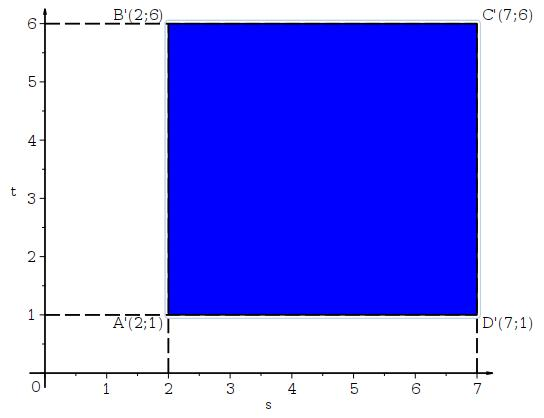
\includegraphics[width=0.3\paperwidth]{example.2.6_1}

Таким чином, область ${D' = h\left(D\right)}$, що є образом області $D$ під дією перетворення $g$, є паралелограм, а фактично --- прямокутник, з вершинами $\left(2,1\right)$, $\left(7,1\right)$, $\left(7,6\right)$ і $\left(2,6\right)$

Для того, щоб застосувати формулу заміни змінних, нам потрібне обернене перетворення $g$. Для того, щоб його отримати, потрібно змінні $x$ і $y$ виразити через змінні $s$ і $t$:

\[
\begin{array}c
\left\{
\begin{array}{l}
s = 3 y - x,\\
t = 2 x - y
\end{array}
\right.
\Leftrightarrow
\left\{
\begin{array}{l}
x = 3 y - s,\\
t = 2 x - y
\end{array}
\right.
\Leftrightarrow
\left\{
\begin{array}{l}
x = 3 y - s,\\
t = 2 \cdot (3 y - s) - y
\end{array}
\right.
\Leftrightarrow
\\[20pt]
\Leftrightarrow
\left\{
\begin{array}{l}
x = 3 y - s,\\
t = 6 y - 2 s - y
\end{array}
\right.
\Leftrightarrow
\left\{
\begin{array}{l}
x = 3 y - s,\\
t = 5 y - 2 s
\end{array}
\right.
\Leftrightarrow
\left\{
\begin{array}{l}
x = 3 y - s,\\
5 y = t + 2 s
\end{array}
\right.
\Leftrightarrow
\\[20pt]
\Leftrightarrow
\left\{
\begin{array}{l}
x = 3 y - s,\\[6pt]
y = \frac{t + 2 s}{5}
\end{array}
\right.
\Leftrightarrow
\left\{
\begin{array}{l}
x = 3 \cdot \frac{t + 2 s}{5} - s,\\[6pt]
y = \frac{t + 2 s}{5}
\end{array}
\right.
\Leftrightarrow
\left\{
\begin{array}{l}
x = \frac{s + 3 t}{5},\\[6pt]
y = \frac{t + 2 s}{5}
\end{array}
\right.
\end{array}
\]
Таким чином, перетворення $g$, обернене до пертворення $h$, задається формулами
\[
\begin{array}{l}
x = \frac{s + 3 t}{5},\\
y = \frac{t + 2 s}{5}.
\end{array}
\]
Знайдемо тепер якобіан:
\[
\begin{array}{c}
J(s, t) = g'(s, t) = \frac{\partial\left(g_1, g_2\right)}{\partial\left(s, t\right)} =
\left|
\begin{array}{cc}
\frac{\partial g_1}{\partial s} & \frac{\partial g_1}{\partial t}\\[6pt]
\frac{\partial g_2}{\partial s} & \frac{\partial g_2}{\partial t}
\end{array}
\right|
=
\begin{vmatrix}
\frac{\partial}{\partial s}\left(\frac{s + 3 t}{5}\right) & \frac{\partial }{\partial t}\left(\frac{s + 3 t}{5}\right)\\[6pt]
\frac{\partial }{\partial s}\left(\frac{t + 2 s}{5}\right) & \frac{\partial }{\partial t}\left(\frac{t + 2 s}{5}\right)
\end{vmatrix}
=\\
=
\left|
\begin{array}{cc}
\frac{1}{5} & \frac{3}{5}\\[6pt]
\frac{2}{5} & \frac{1}{5}
\end{array}
\right|
= \frac{1}{5} \cdot \frac{1}{5} - \frac{3}{5}\cdot \frac{2}{5} = \frac{1}{25} - \frac{6}{25} = -\frac{5}{25} = -\frac{1}{5}.
\end{array}
\]
Згідно з формулою заміни змінних маємо
\[
\begin{array}{c}
\iint\limits_D \ln\left(x + y\right) d x d y = \iint\limits_{D'} \ln\left(\frac{s + 3 t}{5} + \frac{t + 2 s}{5}\right) \cdot\left| -\frac{1}{5} \right| d s d t = \frac{1}{5} \iint\limits_{D'} \ln\frac{3 s + 4 t}{5} d s d t.
\end{array}
\]
Тепер підрахуємо подвійний інтеграл
\[
\iint\limits_{D'} \ln\frac{3 s + 4 t}{5} d s d t.
\]
Оскільки логарифм частки є різницею логарифмів, маємо
\[
\ln\frac{3 s + 4 t}{5} = \ln\left(3 s + 4 t\right) - \ln 5,
\]
і, на підставі лінійності кратних інтегралів,
\[
\iint\limits_{D'} \ln\frac{3 s + 4 t}{5} d s d t = \iint\limits_{D'} \ln\left(3 s + 4 t\right) d s d t - \iint\limits_{D'} \ln 5 d s d t
\]

Інтеграл від константи дорівнює константі, помноженій на міру області інтегрування. В нашому випадку $D'$ є прямокутником, його міра є його площею:
\[
m\left(D'\right) = 5\cdot 5 = 25,
\]
і
\[
\iint\limits_{D'} \ln 5 d s d t = 25\ln 5.
\]
Тепер ми маємо підрахувати подвійний інтеграл
\[
\iint\limits_{D'} \ln\left(3 s + 4 t\right) d s d t.
\]
Останній подвійний інтеграл береться вздовж нової обдасті $D'$, яка є прямокутником, а тому він зводиться до простого повторного інтегралу:
\[
\iint\limits_{D'}\ln\left(3 s + 4 t\right) d s d t = \int\limits_2^7 d s \int\limits_1^6\ln\left(3 s + 4 t\right) d t.
\]
Підрахуємо спочатку
\[
\int\limits_1^6\ln\left(3 s + 4 t\right) d t.
\]
Інтеграл від логарифма рахується за допомогою інтегрування частинами
\[
\int\limits_a^b u dv = u v \biggr|_a^b - \int\limits_a^b v du,
\]
але для спрощення подальших обчислень варто спочатку зробити заміну змінної:
\begin{align*}
&\int\limits_1^6\ln\left(3 s + 4 t\right) d t = &\\[6pt]
&\left(\begin{array}{c}\mbox{ заміна }\\ \mbox{ змінної }\end{array}\right)\left[\begin{array}{c}z = 3 s + 4 t \Leftrightarrow t = \frac{z - 3 s}{4} \\[6pt] dt = \left(\frac{z - 3 s}{4}\right)'_zdz = \frac{dz}{4} \end{array}\ \begin{array}{|c|c|}\hline t&z\\\hline 6&3 s + 24\\\hline 1&3 s + 4\\\hline \end{array}\ \right] = \frac{1}{4}\int\limits_{3 s + 4}^{3 s + 24} \ln z d z = &\\[6pt]
&\left(\begin{array}{c}\mbox{ інтегрівання }\\ \mbox{ частинами }\end{array}\right)\left[\begin{array}{ll}u = \ln z & \ \ \ d v = d z\\ d u = \left(\ln z\right)'d z = \frac{dz }{z} & \ \ \ v = \int dz = z\end{array}\right] = &\\[6pt]
&=\frac{1}{4}\left( z\ln z \biggr|_{3 s + 4}^{3 s + 24} - \int\limits_{3 s + 4}^{3 s + 24}z\cdot\frac{d z}{z}\right) = & \\[6pt]
&\mbox{(підстановка)} &\\[6pt]
&=\frac{1}{4}\left(\left(3 s + 24\right)\ln\left(3 s + 24\right) - \left(3 s + 4\right)\ln\left(3 s + 4\right) - \int\limits_{3 s + 4}^{3 s + 24} d z\right) = & \\[6pt]
&\mbox{(інтеграл від константи)} &\\[6pt]
&=\frac{1}{4}\left(\left(3 s + 24\right)\ln\left(3 s + 24\right) - \left(3 s + 4\right)\ln\left(3 s + 4\right) - \left(3 s + 24 - \left(3 s + 4\right)\right)\right) = & \\[6pt]
&=\frac{1}{4}\left(\left(3 s + 24\right)\ln\left(3 s + 24\right) - \left(3 s + 4\right)\ln\left(3 s + 4\right) - 20\right) &
\end{align*}

Тобто,
\[
\begin{array}{c}
\int\limits_1^6\ln\left(3 s + 4 t\right) d t = \frac{1}{4}\left(\left(3 s + 24\right)\ln\left(3 s + 24\right) - \left(3 s + 4\right)\ln\left(3 s + 4\right) - 20\right).
\end{array}
\]
Таким чином,
\begin{align*}
&\iint\limits_{D'}\ln\left(3 s + 4 t\right) d s d t =&\\
&= \int\limits_2^7 \frac{1}{4}\left(\left(3 s + 24\right)\ln\left(3 s + 24\right) - \left(3 s + 4\right)\ln\left(3 s + 4\right) - 20\right) d s =& \\[6pt]
&\mbox{(лінійність)} &\\[6pt]
&=\frac{1}{4}\int\limits_2^7 \left(\left(3 s + 24\right)\right)\ln\left(3 s + 24\right) d s - \frac{1}{4}\int\limits_2^7 \left(\left(3 s + 4\right)\right) \ln\left(3 s + 4\right) d s - 5 \int\limits_{2}^{7}d s &
\end{align*}
Останній інтеграл від константи, в данному випадку одиниці, дорівнює константі, домноженій на міру множини, тобто, в данному випадку, на довжину проміжка:
\[
 \int\limits_{2}^{7}d s = 1 \cdot \left(7 - 2\right) = 5.
\]
Перші два інтеграли рахуються за допомогою інтегрування частинами. В кожному з них для спрощення обчислень варто спочатку зробити заміну змінної.
\begin{align*}
&\int\limits_2^7 \left(3 s + 24\right)\ln\left(3 s + 24\right) d s = &\\[6pt]
&\left(\begin{array}{c}\mbox{ заміна }\\ \mbox{ змінної }\end{array}\right)\left[\begin{array}{c}z = 3 s + 24 \Leftrightarrow s = \frac{z - 24}{3} \\[6pt] ds = \left(\frac{z - 24}{3}\right)'dz = \frac{dz}{3} \end{array}\ \begin{array}{|c|c|}\hline s&z\\\hline 7 & 45\\\hline 2&30\\\hline \end{array}\ \right] = \frac{1}{3}\int\limits_{30}^{45}z \ln z d z = &\\[6pt]&\left(\begin{array}{c}\mbox{ інтегрівання }\\ \mbox{ частинами }\end{array}\right)\left[\begin{array}{ll}u = \ln z & \ \ \ dv = z d z\\ du = \left(\ln z\right)'dz = \frac{dz}{z} & \ \ \ v = \int z d z = \frac{z^2}{2}\end{array}\right] = &\\[6pt]
&= \frac{1}{3}\left(\frac{z^2}{2}\ln z \biggr|_{30}^{45} - \int\limits_{30}^{45}\frac{z^2}{2}\frac{d z}{z}\right) = & \\[6pt]
&\mbox{(підстановка)} &\\[6pt]
&=\frac{1}{3}\left(\ln 45\cdot \frac{45^2}{2} - \ln 30\cdot \frac{30^2}{2} - \int\limits_{30}^{45}\frac{z}{2} d z =\right)&\\[6pt]
&=\frac{1}{3}\left( \frac{2025}{2}\ln \left(5\cdot 3^2\right) - 450\ln \left(2 \cdot 3 \cdot 5\right) - \int\limits_{30}^{45}\frac{z}{2}d z\right) =&\\[6pt]
&=\frac{1}{3}\left(\frac{2025}{2}\ln 5 + 2025\ln 3 - 450\ln 2 - 450\ln 3 -450 \ln 5 - \frac{z^2}{4}\biggr|_{30}^{45}\right) = &\\[6pt]
&= \frac{1}{3}\left(\frac{1125}{2}\ln 5 + 1575\ln 3 - 450\ln 2 - \left(\frac{45^2}{4} - \frac{30^2}{4} \right)\right) = & \\[6pt]
&=\frac{1}{3}\left( \frac{1125}{2}\ln 5 + 1575\ln 3 - 450\ln 2 - \frac{1125}{4}\right) = & \\[6pt]
&= \frac{375}{2}\ln 5 + 525\ln 3 - 150\ln 2 - \frac{375}{4}.&
\end{align*}
\begin{align*}
&\int\limits_2^7 \left(3 s + 4\right)\ln\left( s + 24\right) d s = &\\[6pt]
&\left(\begin{array}{c}\mbox{ заміна }\\ \mbox{ змінної }\end{array}\right)\left[\begin{array}{c}z = s + 24 \Leftrightarrow s = \frac{z - 4}{3} \\[6pt] ds = \left(\frac{z - 4}{3}\right)'dz = \frac{dz}{3} \end{array}\ \begin{array}{|c|c|}\hline s&z\\\hline 7 & 25\\\hline 2&10\\\hline \end{array}\ \right] = \frac{1}{3}\int\limits_{10}^{25}z \ln z d z = &\\[6pt]&\left(\begin{array}{c}\mbox{ інтегрівання }\\ \mbox{ частинами }\end{array}\right)\left[\begin{array}{ll}u = \ln z & \ \ \ dv = z d z\\ du = \left(\ln z\right)'dz = \frac{dz}{z} & \ \ \ v = \int z d z = \frac{z^2}{2}\end{array}\right] = &\\[6pt]
&= \frac{1}{3}\left(\frac{z^2}{2}\ln z \biggr|_{10}^{25} - \int\limits_{10}^{25}\frac{z^2}{2}\frac{d z}{z}\right) = & \\[6pt]
&\mbox{(підстановка)} &\\[6pt]
&=\frac{1}{3}\left(\ln 25\cdot \frac{25^2}{2} - \ln 10\cdot \frac{10^2}{2} - \int\limits_{10}^{25}\frac{z}{2} d z =\right)&\\[6pt]
&=\frac{1}{3}\left( \frac{625}{2}\ln \left(5^2\right) - 50\ln \left(2 \cdot 5\right) - \int\limits_{10}^{25}\frac{z}{2}d z\right) =&\\[6pt]
&=\frac{1}{3}\left(625\ln 5 - 50\ln 2 - 50 \ln 5 - \frac{z^2}{4}\biggr|_{10}^{25}\right) = &\\[6pt]
&= \frac{1}{3}\left(575\ln 5 - 50\ln 2 - \left(\frac{25^2}{4} - \frac{10^2}{4} \right)\right) = & \\[6pt]
&=\frac{1}{3}\left( 575\ln 5 - 50\ln 2 - \frac{525}{4}\right) = & \\[6pt]
&= \frac{575}{3}\ln 5 - \frac{50}{3}\ln 2 - \frac{175}{4}.&
\end{align*}

Тобто
\begin{align*}
&\int\limits_2^7 \left(3 s + 4\right)\ln\left( s + 24\right) d s = \frac{575}{3}\ln 5 - \frac{50}{3}\ln 2 - \frac{175}{4}.&
\end{align*}

Далі маємо
\begin{align*}
& \iint\limits_{D'}\ln\left(3 s + 4 t\right) d s d t = &\\[6pt]
&= \frac{1}{4}\left(\frac{375}{2}\ln 5 + 525\ln 3 - 150\ln 2 - \frac{375}{4}\right) - \frac{1}{4}\left(\frac{575}{3}\ln 5 - \frac{50}{3}\ln 2 - \frac{175}{4}\right) - 5 \cdot 5 = &\\[6pt]
&=-\frac{25}{24}\ln 5 + \frac{525}{4}\ln 3- \frac{100}{3}\ln 2 - \frac{75}{2},
\end{align*}
потім
\begin{align*}
& \iint\limits_{D'} \ln\frac{3 s + 4 t}{5} d s d t = &\\[6pt]
&=-\frac{25}{24}\ln 5 + \frac{525}{4}\ln 3- \frac{100}{3}\ln 2 - \frac{75}{2} - 25\ln 5 = &\\[6pt]
&=-\frac{625}{24}\ln 5 + \frac{525}{4}\ln 3- \frac{100}{3}\ln 2 - \frac{75}{2},
\end{align*}
і остаточно
\begin{align*}
& \iint\limits_D \ln\left(x + y\right) d x d y = &\\[6pt]
&=\frac{1}{5}\cdot\left(-\frac{625}{24}\ln 5 + \frac{525}{4}\ln 3- \frac{100}{3}\ln 2 - \frac{75}{2}\right) = -\frac{125}{24}\ln 5 + \frac{105}{4}\ln 3- \frac{20}{3}\ln 2 - \frac{15}{2}.
\end{align*}


\end{example}















